%\documentclass[letterpaper, 10 pt, conference]{ieeeconf}`
%\usepackage{filecontents,lipsum}
%\usepackage[noadjust]{cite}
%%\begin{filecontents*}{references.bib}
%%@article{Khoe:1994:CML:2288694.2294265,
%%    author = {Khoe, G. -D.},
%%    title = {Coherent multicarrier lightwave technology for flexible capacity networks},
%%    journal = {Comm. Mag.},
%%    issue_date = {March 1994},
%%    volume = {32},
%%    number = {3},
%%    month = mar,
%%    year = {1994},
%%    issn = {0163-6804},
%%    pages = {22--33},
%%    numpages = {12},
%%    url = {http://dx.doi.org/10.1109/35.267438},
%%    doi = {10.1109/35.267438},
%%    acmid = {2294265},
%%    publisher = {IEEE Press},
%%    address = {Piscataway, NJ, USA},
%%}
%%\end{filecontents*}
%\title{This document}
%\author{This author}

%%%%%%%%%%%%%%%%%%%%%%%%%%%%%%%%%%%%%%%%%%%%%%%%%%%%%%%%%%%%%%%%%%%%%%%%%%%%%%%%
%2345678901234567890123456789012345678901234567890123456789012345678901234567890
%        1         2         3         4         5         6         7         8

\documentclass[letterpaper, 10 pt, conference]{ieeeconf}  % Comment this line out if you need a4paper

%\documentclass[a4paper, 10pt, conference]{ieeeconf}      % Use this line for a4 paper

\IEEEoverridecommandlockouts                              % This command is only needed if 
                                                          % you want to use the \thanks command

\overrideIEEEmargins                                      % Needed to meet printer requirements.

% See the \addtolength command later in the file to balance the column lengths
% on the last page of the document

% The following packages can be found on http:\\www.ctan.org
%\usepackage{graphics} % for pdf, bitmapped graphics files
%\usepackage{epsfig} % for postscript graphics files
%\usepackage{mathptmx} % assumes new font selection scheme installed
%\usepackage{times} % assumes new font selection scheme installed
%\usepackage{amsmath} % assumes amsmath package installed
%\usepackage{amssymb}  % assumes amsmath package installed
%\usepackage{filecontents,lipsum}
%\usepackage[noadjust]{cite}
%\usepackage{bm}
%\usepackage{tikz}
%\usepackage{graphicx}
%\usepackage{caption}
%\usepackage{subcaption}
%\usepackage{multicol}
%\usepackage{url}
%\usepackage{geometry}
%\usepackage{mathtools}
%\usepackage[utf8]{inputenc}
%\usepackage[english]{babel}
%\usepackage{algorithm}
%\usepackage[]{algpseudocode}


\usepackage{afterpage}
\usepackage{algorithm}
\usepackage[]{algpseudocode}

\usepackage{stix}
\usepackage{amssymb}
\usepackage{amsmath}

\DeclareMathAlphabet\mathbfcal{OMS}{cmsy}{b}{n}
%\usepackage[math-style=TeX, bold-style=TeX]{unicode-math}

\usepackage{arydshln}
\usepackage[english]{babel}
\usepackage{bm}
\usepackage{caption}
\usepackage[T1]{fontenc}
\usepackage[]{graphicx}
\graphicspath{ {./fig/} }

\usepackage[utf8]{inputenc}
\usepackage{multicol}
\usepackage[T1]{xcolor}
\usepackage{soul}
\usepackage{subfig}
\usepackage{tikz}
\usepackage{url}
\usepackage[backend=biber,style=ieee,sorting=none]{biblatex}
\addbibresource{bib/references.bib}

\newcommand{\trsp}{{^{\top}}}

\newcommand\blankpage{%
    \null
    \thispagestyle{empty}%
    \addtocounter{page}{-1}%
    \newpage}



\newcommand*{\important}[1]{\textcolor{red}{\danger~\textbf{IMPORTANT:~}} \textcolor{red}{#1}}

\newcommand*{\pending}[1]{\textcolor{blue}{$\bigstar$~\textbf{PENDING~#1}}}

\newcommand\mybox[2][]{\tikz[overlay]\node[fill=blue!100,inner sep=4pt, anchor=text, rectangle, rounded corners=1mm,#1] {#2};\phantom{#2}}

\newcommand{\TODO}{\mybox[fill=yellow]{\textcolor{blue}{\Large \textbf{TODO}}}}
\newcommand\myhl[1]{\textcolor{red}{#1}}


\newtheorem{prop}{Proposition}

\usepackage[nolist]{acronym}
\newacro{smc}[SMC]{sensorimotor contingencies}
\newacro{dfc}[DFC]{dynamic functional connectivity}
\newacro{fc}[FC]{functional connectivity}
\newacro{nnmf}[NNMF]{non-negative matrix factorization}
\newacro{imi}[IMI]{instantaneous mutual information}
\newacro{irm}[IRM]{infinite realtional model}

\newacro{}[]{}
\newacro{}[]{}
\newacro{}[]{}

\title{\LARGE \bf
Dynamic sensorimotor graphs
}


\author{Valentin Marcel, Fernando D\'iaz Ledezma, Matej Hoffmann}

\begin{document}

\maketitle

\begin{abstract}
\myhl{Regularities present in the somatosensory signals of a robotic agent can reflect its embodiment and the associations resulting from an active control policy. In this work, we analyze the dynamic functional connectivity of the somatosensory signals based on the instantaneous pairwise mutual information. As the robot performs exploratory motions based on motor babbling, we capture and study the time-varying changes in the signal relationships. We analyze the instantaneous and average information sharing and associate them with different information states. A simulated planar system study shows that using instantaneous mutual information to extract and leverage the relationships between the agent's somatosensory signals exhibited during exploratory motions can yield information related to self-touch events.}
\end{abstract}
% =============================================================================
%                                                                             |
%                                                                             |
% ------------------------------- SECTION ------------------------------------|
%                                                                             |
%                                                                             |
% =============================================================================

\section{Introduction}\label{sec:intro}
Understanding the brain’s structural and \ac{fc} has significantly advanced our knowledge of its organization and information-processing capabilities. A similar approach can be applied to studying the sensorimotor signals of an embodied agent, offering insights into how the agent processes information and adapts its behavior. While analyzing the structural connectivity of these signals may not always be feasible, investigating their functional connectivity provides a powerful way to understand an agent’s body structure and the emergence of behavior through information acquisition. A key concept in this context is that of \ac{smc} \cite{Jacquey2019Sensorimotorcontingenciesas}, the regularities and dependencies between an organism's actions (motor actions) and the resulting sensory feedback linking an agent’s sensorimotor signals to its physical embodiment and the world. Identifying and analyzing these regularities using information-theoretic methods can help uncover fundamental principles of sensorimotor learning. 
% ---
\begin{figure}[!ht]
	\centering
	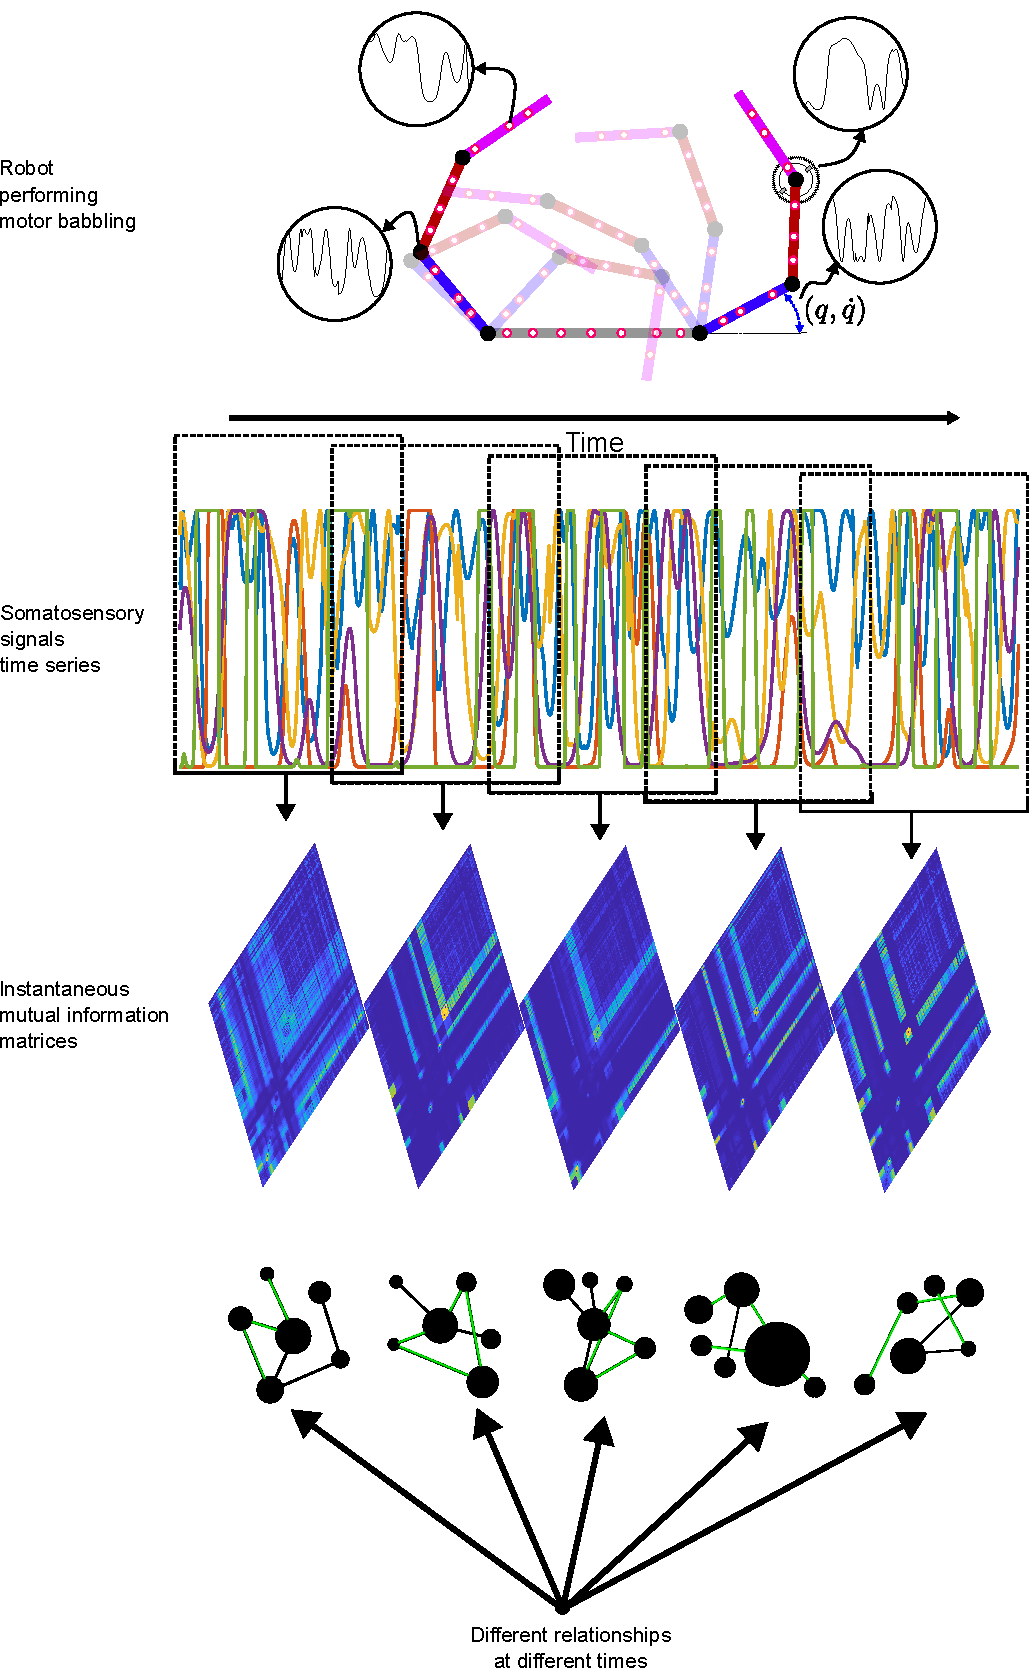
\includegraphics[width=0.9\columnwidth]{somatosensry_dynamic_functional_connectivity.pdf}
	\caption{\textbf{General overview.} Motion excites the sensorimotor system of a robotic agent. While moving, the sensorimotor functional connectivity changes over time.}
	\label{fig:general_overview}
\end{figure}
% ---

% SUBSECTION ==================================================================
\subsection{Related works}
Research suggests that \acp{smc} play a fundamental role in acquiring body knowledge, generalization, and goal-directed behavior \cite{Jacquey2019Sensorimotorcontingenciesas}. As such, they can be viewed as a form of sensorimotor representation---a framework that enables an embodied agent to learn, adapt, and interact with its environment. Despite extensive research on sensorimotor representations \cite{Nguyen2021Sensorimotorrepresentationlearning}, the precise relationship between sensorimotor regularities, body knowledge, and behavior remains an open question.

Several studies have used information-theoretic metrics to examine these relationships in sensorimotor systems \cite{Schmidt2013Bootstrappingperceptionusing,Lungarella2006Mappinginformationflow,Polani2009Modelsinformationprocessing,Bossomaier2016introductiontransferentropy,Olsson2006unknownsensorsactuators}. Among different sensory modalities, touch has been identified as particularly crucial in understanding \acp{smc}. For example, Gama et al. \cite{Gama2021Goaldirectedtactile} demonstrated how intrinsic motivation and goal-babbling can facilitate self-touch learning in a simulated humanoid robot with artificial tactile skin. Similarly, Roncone et al. \cite{Roncone2014Automatickinematicchain} showed that self-touch could be used for kinematic calibration, allowing a robot to close its kinematic chain autonomously by touching its own body. Marcel et al. \cite{Marcel2022Learningreachown} further explored self-touch representation using a denoising framework with a multimodal variational autoencoder, enabling a robot to reconstruct its self-reaching configurations internally.

Another relevant area of study is \ac{dfc}, which explores how the statistical properties of sensorimotor signals evolve over time. Originally applied in neuroscience, \ac{dfc} has been used to detect states of reduced functional connectivity during epilepsy onsets \cite{Christiaen2020Dynamicfunctionalconnectivity} and to identify abnormal connectivity patterns in brains affected by illness \cite{Zhou2020Earlychildhooddevelopmental}. More recently, \ac{dfc} has been used to investigate how sensorimotor connectivity evolves in simulated infants as they develop \cite{Kanazawa2023Openendedmovements}.

In robotics, functional connectivity is expected to change based on the robot’s motion policy or the task it performs. Capturing and analyzing these evolving patterns using \ac{dfc} could provide a deeper understanding of how an agent’s sensory and motor systems interact over time.
% SUBSECTION ==================================================================
\subsection{Contribution}
This work investigates the time-varying functional connectivity between the visual, tactile, and proprioceptive signals of a simulated two-dimensional embodied agent. As the agent moves, its motor policy influences its sensorimotor connectivity, creating dynamic patterns that can be represented as evolving graphs. Our approach leverages dynamic functional connectivity to study the formation and evolution of \acp{smc}.

To achieve this, we analyze instantaneous pairwise mutual information, revealing how the agent’s information-sharing state correlates with its motion and potential self-interactions. By applying non-negative matrix factorization (NMF), we extract distinct information-sharing states and classify them based on their informational content.

After a motor babbling phase, we demonstrate that—without prior knowledge of the agent’s morphology—the different information states and their transitions reveal essential aspects of the agent’s body structure and behavior.
\myhl{In this work, we study the time-varying functional connections between visual, tactile, and proprioceptive signals of a simulated two-dimensional embodied agent. Given that the motor policy changes the sensorimotor connectivity of the agent, we capture the varying connectivity patterns as dynamic graphs. The ensuing \ac{dfc} helps understand the formation and evolution of \acp{smc}. We achieve this by looking at the instantaneous pairwise mutual information, showing how the agent's information-sharing state is related to its motion and consequent potential interaction with itself. Using non-negative matrix factorization, we extract different information-sharing states and classify them according to their information content. After a motor babbling phase, we show how, by focusing only on the mutual information and without a priori knowledge about the agent's morphology, the different information states, and associated transitions reveal aspects of the agent's embodiment.}

% =============================================================================
%                                                                             |
%                                                                             |
% ------------------------------- SECTION ------------------------------------|
%                                                                             |
%                                                                             |
% =============================================================================
% ---
\begin{figure}[!t]
	\begin{center}
		\hspace*{\fill}
		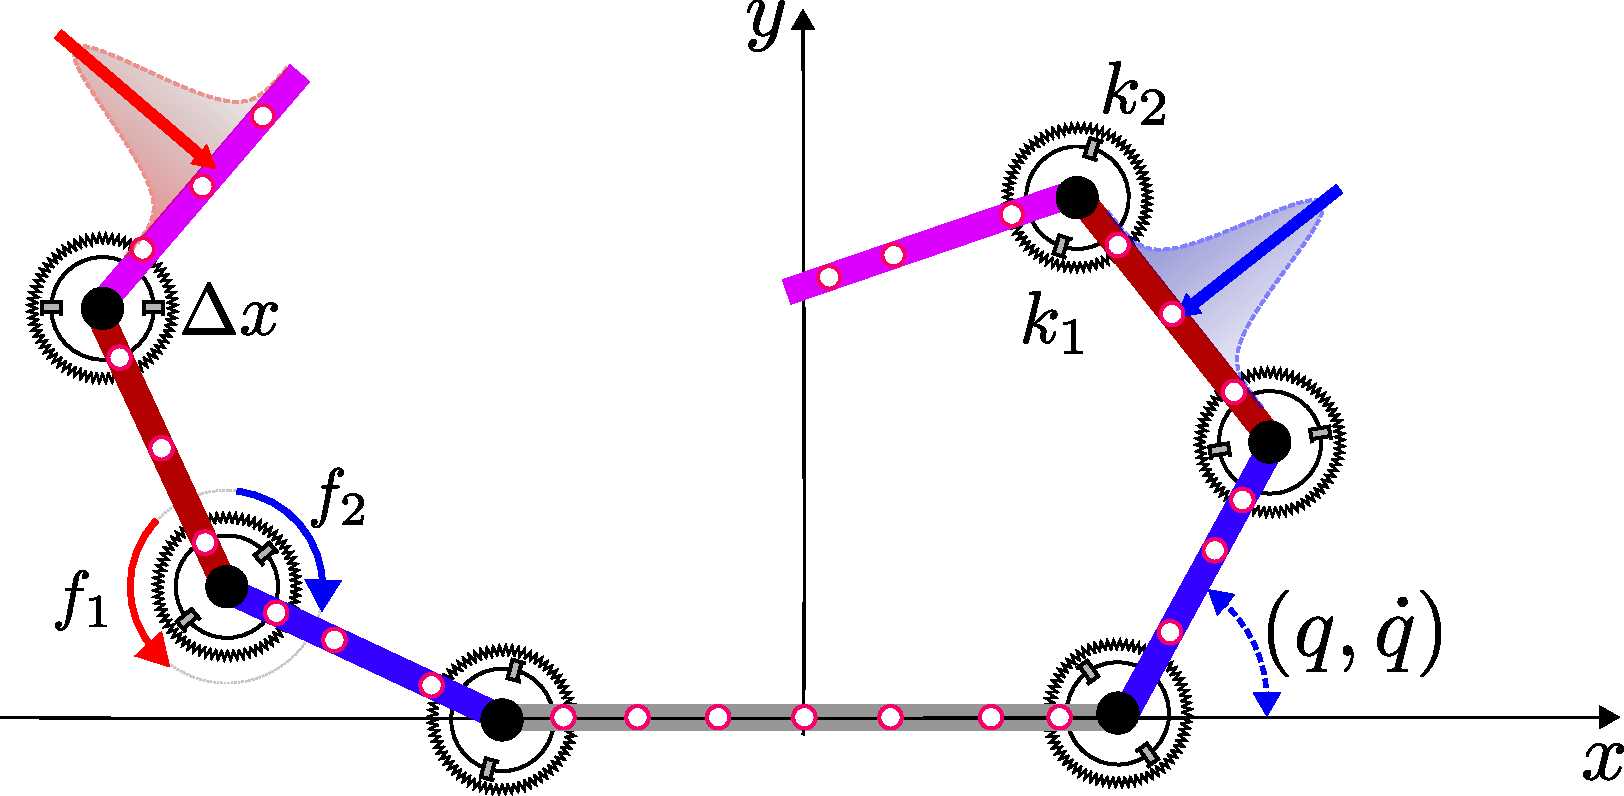
\includegraphics[width=0.99\columnwidth]{extended_dual_arm_robot.pdf}
		\hspace*{\fill}
	\end{center}
	\caption{\label{fig:extended_dual_arm_robot} \textbf{The embodied agent.} The planar dual arm robot with antagonistic actuation.}
\end{figure}
% ---
\section{The embodied agent}

% SUBSECTION ==================================================================
\subsection{The planar dual arm model}
We employ the robot model described in \cite{Mannella2018Knowyourbody,Marcel2022Learningreachown} as our reference system. This model consists of a simple planar dual-arm system with six degrees of freedom, featuring three links per arm and a fixed torso, see Fig.~\ref{fig:extended_dual_arm_robot}. The robot is equipped with tactile sensors distributed across its body. To instantiate the dynamics of the model, inertial properties are assigned to the robot's composing bodies. Its actuation mechanism is based on a biology-inspired model presented in \cite{Ekeberg1993combinedneuronalmechanical,Wadden1998neuromechanicalmodel, Shim2012Chaoticexplorationlearning}, where the position $q$ and velocity $\dot{q}$ of each joint is driven by antagonistic muscles (modeled as spring-damper systems). The pulling force these muscles exert is linearly controlled by the signal generated by a corresponding motor neuron $\sigma$. The joint torque,
% ---
\begin{equation}\label{eq:antagonistic_torque}
	\tau = \alpha \left(\sigma_\mathrm{fx} - \sigma_\mathrm{ex}\right)  + \beta \left(\sigma_\mathrm{fx} + \sigma_\mathrm{ex} + \gamma \right) q + \delta \dot{q},
\end{equation}
% ---
results from the difference between activation signals for flexion $ \sigma_\mathrm{fx} $ and extension $\sigma_\mathrm{ex}$. These activation signals contribute to the flexion and extension pulling forces, $ f_\mathrm{fx}$ and $f_\mathrm{ex} $, respectively. The remaining parameters in the model account for the muscle force gain ($\alpha$), stiffness gain ($\beta$), tonic stiffness ($\gamma$), and damping coefficient ($\delta$).

% SUBSECTION ==================================================================
\subsection{The sensory signals}
Randomly located tactile sensors along the robot's one-dimensional body are modeled based on population coding \cite{Panzeri2010PopulationCoding}. They are represented as distance-dependent Gaussian receptive fields---see Fig.~\ref{fig:population_coding}---whose mean is dictated by the tactile sensor location. 
To incorporate touch strength into the model, we adjust the distance-based activation of the Gaussian receptive fields based on the contact force. Similarly, the proprioceptive measurements of the robot are also encoded using receptive fields. Ultimately, our extended model results in a vector $\bm{s}$ containing a number $N_s$ of somatosensory signals encompassing proprioception (joint position $\bm{p}$, velocity $\bm{v}$, and effort $\bm{e}$) and touch-strength-modulated tactile signals $\bm{r}$; i.e.:
% ---
\begin{equation}
	\bm{s} = \begin{bmatrix}
		\bm{p}\trsp & \bm{v}\trsp & \bm{e}\trsp & \bm{r}\trsp
	\end{bmatrix}\trsp \in \mathbb{R}^{N_s}_{\geq}.
\end{equation}
%---
\myhl{In addition to somatosensation, we equip the robot with visual inputs. The visual sensors are composed of a fixed, rectangular, pixel grid of size $(s_\text{x},s_\text{y})$ with  $(n_\text{x},n_\text{y})$ pixels in each direction. Pixels are sensitive to the positions of the agent's limbs; e.g., when a limb segment intersects with the rectangular pixel receptive field in the 2D space, its value is updated to one. To simulate some visual sensors' spatial overlap~\cite{Marshall2015}, we perform a convolution of the pixel values image with a 3-by-3 kernel mapping to get the visual sensors' activations.}

%\begin{figure*}[htp!]
%	\centering	
%	\hspace*{\fill}
%	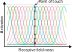
\includegraphics[width= 0.6\textwidth]{fig/receptive_fields.pdf}
%	\hspace*{\fill}
%	\caption[] {\label{fig:receptive_fields} The Gaussian receptive fields used in population coding.}
%\end{figure*}



% ---
\begin{figure}[!t]
	\begin{center}
		\hspace*{\fill}
		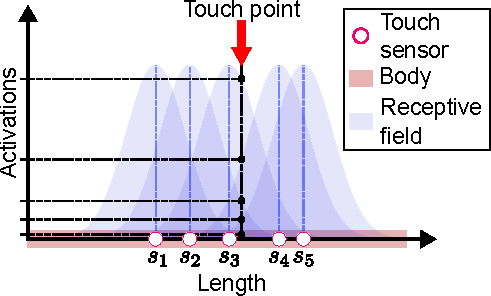
\includegraphics[width=0.99\columnwidth]{touch_receptive_fields.pdf}
		\hspace*{\fill}
	\end{center}
	\caption{\label{fig:population_coding} \textbf{Population coding.} The receptive fields encode a signal into several distance-based activation functions.}
\end{figure}
% ---
% =============================================================================
%                                                                             |
%                                                                             |
% ------------------------------- SECTION ------------------------------------|
%                                                                             |
%                                                                             |
% =============================================================================
\section{The sensorimotor dynamic functional connectivity}

% Subsection ==================================================================
\subsection{Functional connectivity}
\ac{fc} is a method for network topology inference that characterizes the dependencies of the observed signals from a system based on their probability distributions \cite{Friston2011Functionaleffectiveconnectivity}. It can be subdivided into undirected and directed, the latter being related to the analysis of statistical causation from the data \cite{Bastos2016tutorialreviewfunctional}. By studying the \ac{fc}, it is possible to reveal a structure that aids in analyzing the interaction among the entities in a network.

Based on the connection between embodiment and information structure \cite{Pfeifer2007Selforganizationembodiment}, we hypothesize that properties of the sensorimotor interactions can be made apparent by studying the \ac{fc} among the bodily signals $ \bm{s}(t) $. From the various metrics that have been proposed to evaluate such relationships, we, in particular, leverage those based on information theory \cite{Bonsignorio2020EntropyBasedMetrics,Bonsignorio2013Quantifyingevolutionaryself}, as their model-free nature can capture linear and nonlinear relationships between signals. Particularly, we use mutual information (MI), a quantity that has been applied in different contexts to quantify the relationships between variables \cite{Steuer2002mutualinformationdetecting}. The MI between two signals $ I\left(X;Y\right) $ can be interpreted as the amount by which a random signal $ Y $ reduces the uncertainty about a random signal $ X $ \cite{Cover1999Elementsinformationtheory}. It is a symmetric measure of the information sharing by both signals and is computed as:
% ---
\begin{equation}\label{eq:mutual_information}
	I\left(X;Y\right) =I\left(Y;X\right) = H(X) + H(Y) - H(X,Y),
\end{equation}
% ---
Using $p(\cdot)$ and $p(\cdot,\cdot)$ to denote the marginal and joint probability distributions, the Shannon's entropy of a variable $X$ is defined by 
% ---
\begin{equation}\label{eq:entropy}
	H(X) = -\sum_{i=1}^{n}p(x_i)\text{log}_2\left(p\left(x_i\right)\right)
\end{equation}
% ---
and the joint entropy between $ X $ and $ Y $ expressed as
% ---
\begin{equation}\label{eq:joint_entropy}
	H(X,Y) = -\sum_{i=1}^{n}\sum_{j=1}^{n} p(x_i,y_j)\text{log}_2\big(p\left(x_i,y_j\right)\big).
\end{equation}
% ---
By extension, the mutual information matrix $\bm{\mathcal{I}} \in \mathbb{R}^{{N_s} \times {N_s}}$ can be constructed by computing the pairwise MI between the $\left\lbrace s_i\right\rbrace^{N_s}_{i=1}$ sensorimotor signals. In practice, computing an entry
% ---
\begin{equation}\label{eq:adjacency_mi}
	\left(\bm{\mathcal{I}}\right)_{i,j} = I(s_i;s_j)
\end{equation}
% ---
for a pair $\left({s}_i(t),{s}_j(t)\right)$ involves centering their samples---to zero mean and unit standard deviation---and using either binning, kernel, or nearest neighbor methods \cite{WaltersWilliams2009Estimationmutualinformation} to compute their mutual information. In this work, for the computation of $\bm{\mathcal{I}}$, we use the open-source MATLAB package \emph{Mutual information computation} \cite{PengMutualInformationcomputation}.

% Subsection ==================================================================
\subsection{Dynamic functional connectivity}
When analyzing \ac{fc}, it might be interesting to look at the aggregated effect of a complete dataset of recordings and the instantaneous changes that occur in the relationships. Indeed, the functional relationships between sensorimotor signals can change rapidly depending on the motion policy and the agent's interaction with the environment. To capture this time-varying, i.e., dynamic, functional connectivity with mutual information, it is common to use a sliding time window \cite{Preti2017dynamicfunctionalconnectome} with forward step $\Delta t$ from which the MI is computed only for a small number of samples.

For a time window of length $T$, the mutual information $I_t(s_x(t);s_y(t))$ between a distinct pair of signals $s_x(t)$ and $s_y(t)$ at time $t$ is computed using the set of signal samples spanning the $\left[t-T,t\right]$ interval\footnote{The selection of a relatively short time window is motivated by the fact that tactile events often occur within a short timescale.}, as illustrated in Fig.~\ref{fig:mi_sliding_window_mi}. We refer to this quantity as the \ac{imi}. 

Extending this concept, the mutual information matrix $\bm{\mathcal{I}}(t)$ at time $t$ is constructed by calculating the \ac{imi} for all pairwise signals within the same time interval. The temporal evolution of this time-varying mutual information matrix $\bm{\mathcal{I}}(t)$ captures the dynamic functional connectivity between the sensorimotor signals.
% ---
\begin{figure}[!t]
	\begin{center}
		\hspace*{\fill}
		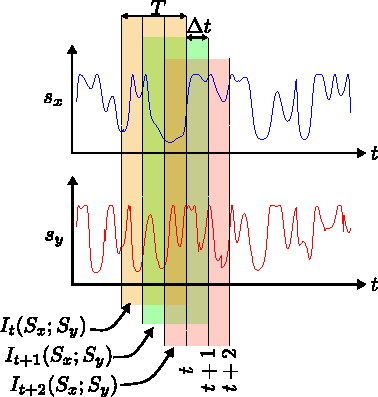
\includegraphics[width=0.99\columnwidth]{sliding_window_mi.pdf}
		\hspace*{\fill}
	\end{center}
	\caption{\label{fig:mi_sliding_window_mi} \textbf{Instantaneous mutual information.} A sliding window strategy is used to compute the \ac{imi} in an interval  $\left[t-T,t\right]$.}
\end{figure}
% ---

% Subsection ==================================================================
\subsection{Finding structure in the relationships}
The \ac{irm} is a probabilistic framework designed to identify hidden structures in relational data; that is, data that captures relationships between entities. It is based on clustering entities (e.g., nodes in a graph) into groups while simultaneously learning relationships between them. Its primary objective is to group entities into clusters based on their relationships and predict new relationships based on these assignments. Unlike traditional models that require a fixed number of clusters, the IRM employs a Bayesian nonparametric approach (typically a Chinese Restaurant Process or a Dirichlet Process), allowing the number of clusters to grow dynamically as needed. This flexibility makes it particularly useful for analyzing complex datasets with unknown group structures. By leveraging probabilistic methods, the IRM estimates the likelihood of entities belonging to the same cluster and models inter-cluster relationships using probability distributions. Since exact inference is intractable, \ac{irm} uses Gibbs sampling, a Markov Chain Monte Carlo method, to iteratively refine cluster assignments and relationship probabilities. Entities are re-assigned to clusters based on how well they fit the observed relationships.

To our purposes, the \ac{irm} receives as an input the time series of $\bm{\mathcal{I}}$ matrices and assigns to each of the nodes $i$ ---i.e., each sensorimotor signal---a cluster $z_i$. To find these latent cluster relationships, \ac{irm} assumes that the probability of a relation between two entities depends only on their cluster memberships. If two entities belong to clusters $z_i$ and $z_j$, the probability of a connection is given by a parameter $\theta_{z_i,z_j}$.
These inter-cluster probabilities form a relationship matrix, which the model infers from data. These inter-cluster probabilities form a relationship matrix, which the model infers from data.

The final result is:
\begin{itemize}
    \item A clustering of entities into groups.
    \item A learned block matrix showing the probability of relations between clusters.
\end{itemize}


% Subsection ==================================================================
\subsection{Analyzing recurring patterns}
Given a set of $m$ samples from the somatosensory signals generated, for example, via motor babbling, a dataset $\bm{S} \in \mathbb{R}^{n \times m}_{\geq}$ can be used to search for repeating patterns of \ac{fc} that encode certain modes of operation. It is also important to determine these patterns' strength and frequency of expression to determine their relevance. Typical methods to detect repeating patterns in dynamic \ac{fc} include the cosine similarity \cite{Menon2019comparisonstaticdynamic}, k-means clustering\cite{Li2017Hightransitionfrequencies}, and  \ac{nnmf} \cite{Fu2019Nonnegativematrixfactorization}. We chose the latter, as it has proven useful in several studies analyzing brain dynamic functional networks and has also been used for community  detection\cite{Wang2011Communitydiscoveryusing,Luo2021Symmetricnonnegativematrix}.

\ac{nnmf} is an unsupervised machine learning algorithm that can be used to split an input matrix $\bm{D}_{\bm{\mathcal{I}}} \in \mathbb{R}^{n\times m}_{\geq}$ into two parts: a matrix $\bm{W} \in \mathbb{R}^{n\times k}_{\geq}$ of bases and a matrix $\bm{H} \in \mathbb{R}^{k\times m}_{\geq}$ of their corresponding contributions to the input matrix $\bm{D}_{\bm{\mathcal{I}}}$; i.e.,
% ---
\begin{equation}
	\bm{D}_{\bm{\mathcal{I}}} 	\approx \bm{W} \bm{H}.
\end{equation}
% ---
\begin{figure}[!t]
	\centering
	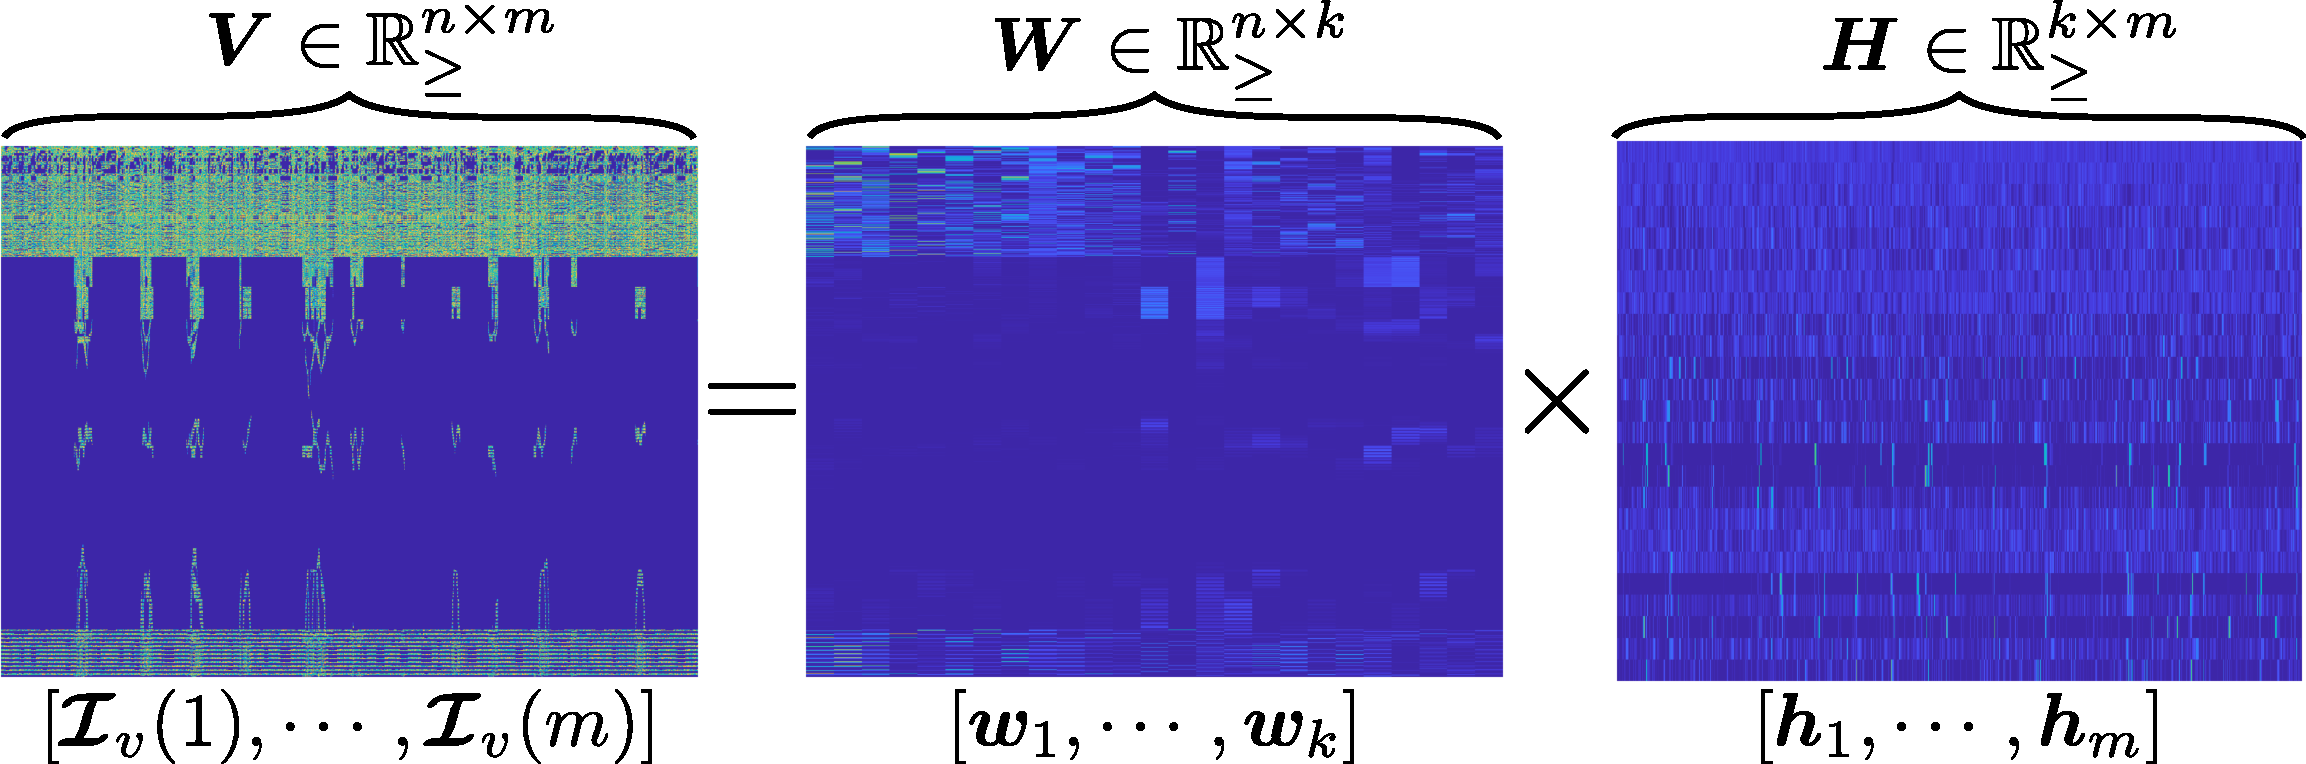
\includegraphics[width=0.99\columnwidth]{fig/nnmf_concept.pdf}
	\caption{\textbf{Non-negative matrix factorization.} Decomposition of the \ac{imi} data matrix $\bm{S}$ using \ac{nnmf} helps identifying recurring patterns.}
	\label{fig:nnmf}
\end{figure}
% ---
In our case, the matrix $\bm{D}_{\bm{\mathcal{I}}}$ is constructed by vectorizing  and concatenating each of the matrices $\bm{\mathcal{I}}_v(t) = \text{vec}\left(\bm{\mathcal{I}}(t)\right)$; that is, 
\begin{equation}
	\bm{D}_{\bm{\mathcal{I}}} = [\bm{\mathcal{I}}_v(1),\cdots,\bm{\mathcal{I}}_v(m)].
\end{equation}
Note that $n = N_s(N_s-1)/2$ is the total number of mutual information pairs. Since the matrix $D_{\bm{\mathcal{I}}}$ is strictly non-negative, it is amenable to be decomposed and analyzed using \ac{nnmf}. One crucial question is the number of factors $k$ used to approximate the original dataset. From the various methods to select an adequate number \cite{Muzzarelli2019RankSelectionNon}, we chose $k$ following the elbow method as in \cite{Phalen2020Nonnegativematrix} by performing \ac{nnmf} for ascending values of $k$ and selecting the value where the residual error is not reduced any further.

Each of the factors $\left\lbrace\bm{w}_i\right\rbrace^k_i=1$ can be interpreted as a base \ac{fc} graph capturing
a state of information sharing of multiple sensorimotor states. When the factors are aggregated using via the columns of $\bm{H}$, the particular mutual information matrix at time $t$ is closely approximated.

%It is worth mentioning that \ac{nnmf} is an stochastic method and thus, two different runs will produce two distinct set of factors. 
To facilitate the analysis of the relevance of each of the factors, after factorization, the factors are normalized according to the $L_2$-norm. 

% XXXXXXXXXXXXXXXXXXXXXXXXXXXXXXXXXXXXXXXXXXXXXXXXXXXXXXXXXXXXXXXXXXXXXXXXXXXXXX
%Intuitively, NMF decomposes functional brain networks into the following: (1) a set of subnetworks (patterns) overlapping in space and
%time and (2) corresponding coefficient time series that quantify the
%contribution of each subnetwork (pattern) at each time point
%(Chai et al., 2017; Khambhati et al., 2017, 2018a,b). 
%
%As compared to
%hard-partitioning schemes, the advantage of this method is that it
%provides information about brain-network dynamics in a continuous,
%overlapping manner in space and time rather than in discrete partitions.
%Furthermore, owing to the parts-based nature of the technique, we
%obtained subnetworks that resembled the localized features of largescale brain networks rather than generalized patterns of the overall
%network
% XXXXXXXXXXXXXXXXXXXXXXXXXXXXXXXXXXXXXXXXXXXXXXXXXXXXXXXXXXXXXXXXXXXXXXXXXXXXXX

%In \cite{Stiso2020Learningbraincomputer} it is shown how the basis graph change their expressing during learning of a task



% =============================================================================
%                                                                             |
%                                                                             |
% ------------------------------- SECTION ------------------------------------|
%                                                                             |
%                                                                             |
% =============================================================================
\section{Simulation results}

% ---
\begin{figure}[!th]
	\begin{center}
		\hspace*{\fill}
		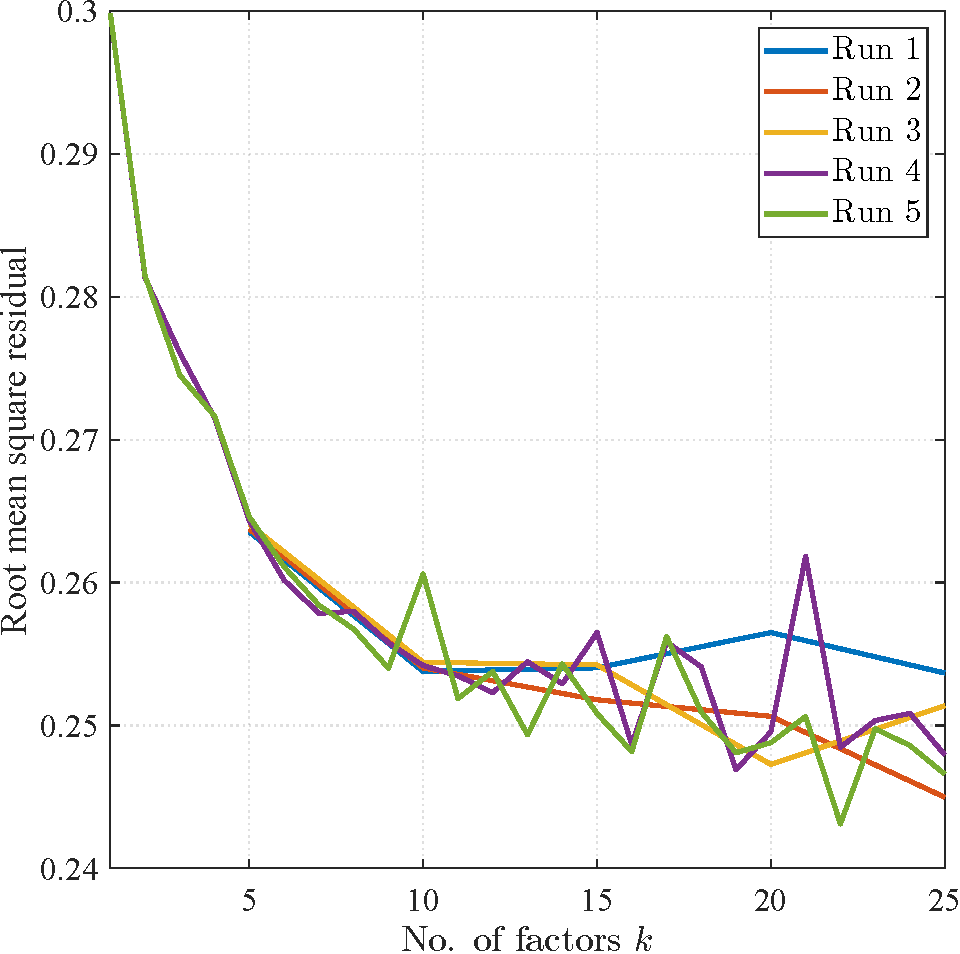
\includegraphics[width=0.99\columnwidth]{nnmf_elbow.pdf}
		\hspace*{\fill}
	\end{center}
	\caption{\label{fig:nnmf_elbow} Elbow method to determine the number of factors for \ac{nnmf}.}
\end{figure}
% ---

\subsection{Exploratory phase}
\begin{figure*}[!ht]
	\centering
	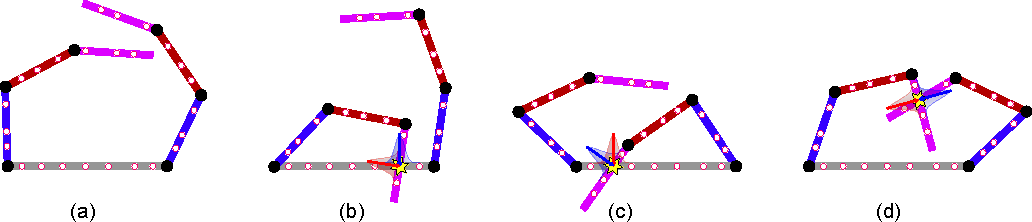
\includegraphics[width=0.9\textwidth]{planar_dual_arm_modes.pdf}
	\caption{Different events during exploration. (a) Pure proprioception (no touch), (b) contact with left arm, (c) contact with right arm, and (d) contact with both arms.}
	\label{fig:planar_dual_arm_modes}
\end{figure*}
% ---
For the computation of the instantaneous mutual information, we used sensor signals sampled at 100 Hz and a sliding window of $T = 0.1$ seconds, i.e., the previously seen 10 samples. With this short memory which is stored in a buffer, we can capture (fast) touch events.

% Subsection ==================================================================
\subsection{Dimensionality reduction}
To show graphically how the different factors cluster naturally depending on the touched regions, we used the PaCMAP dimensionality reduction method \cite{Wang2021Understandinghowdimension} given its properties to preserve aspects of the global and local structure when reducing into the latent space \cite{Huang2022Towardscomprehensiveevaluation}.

\begin{figure}[!th]
	\centering
	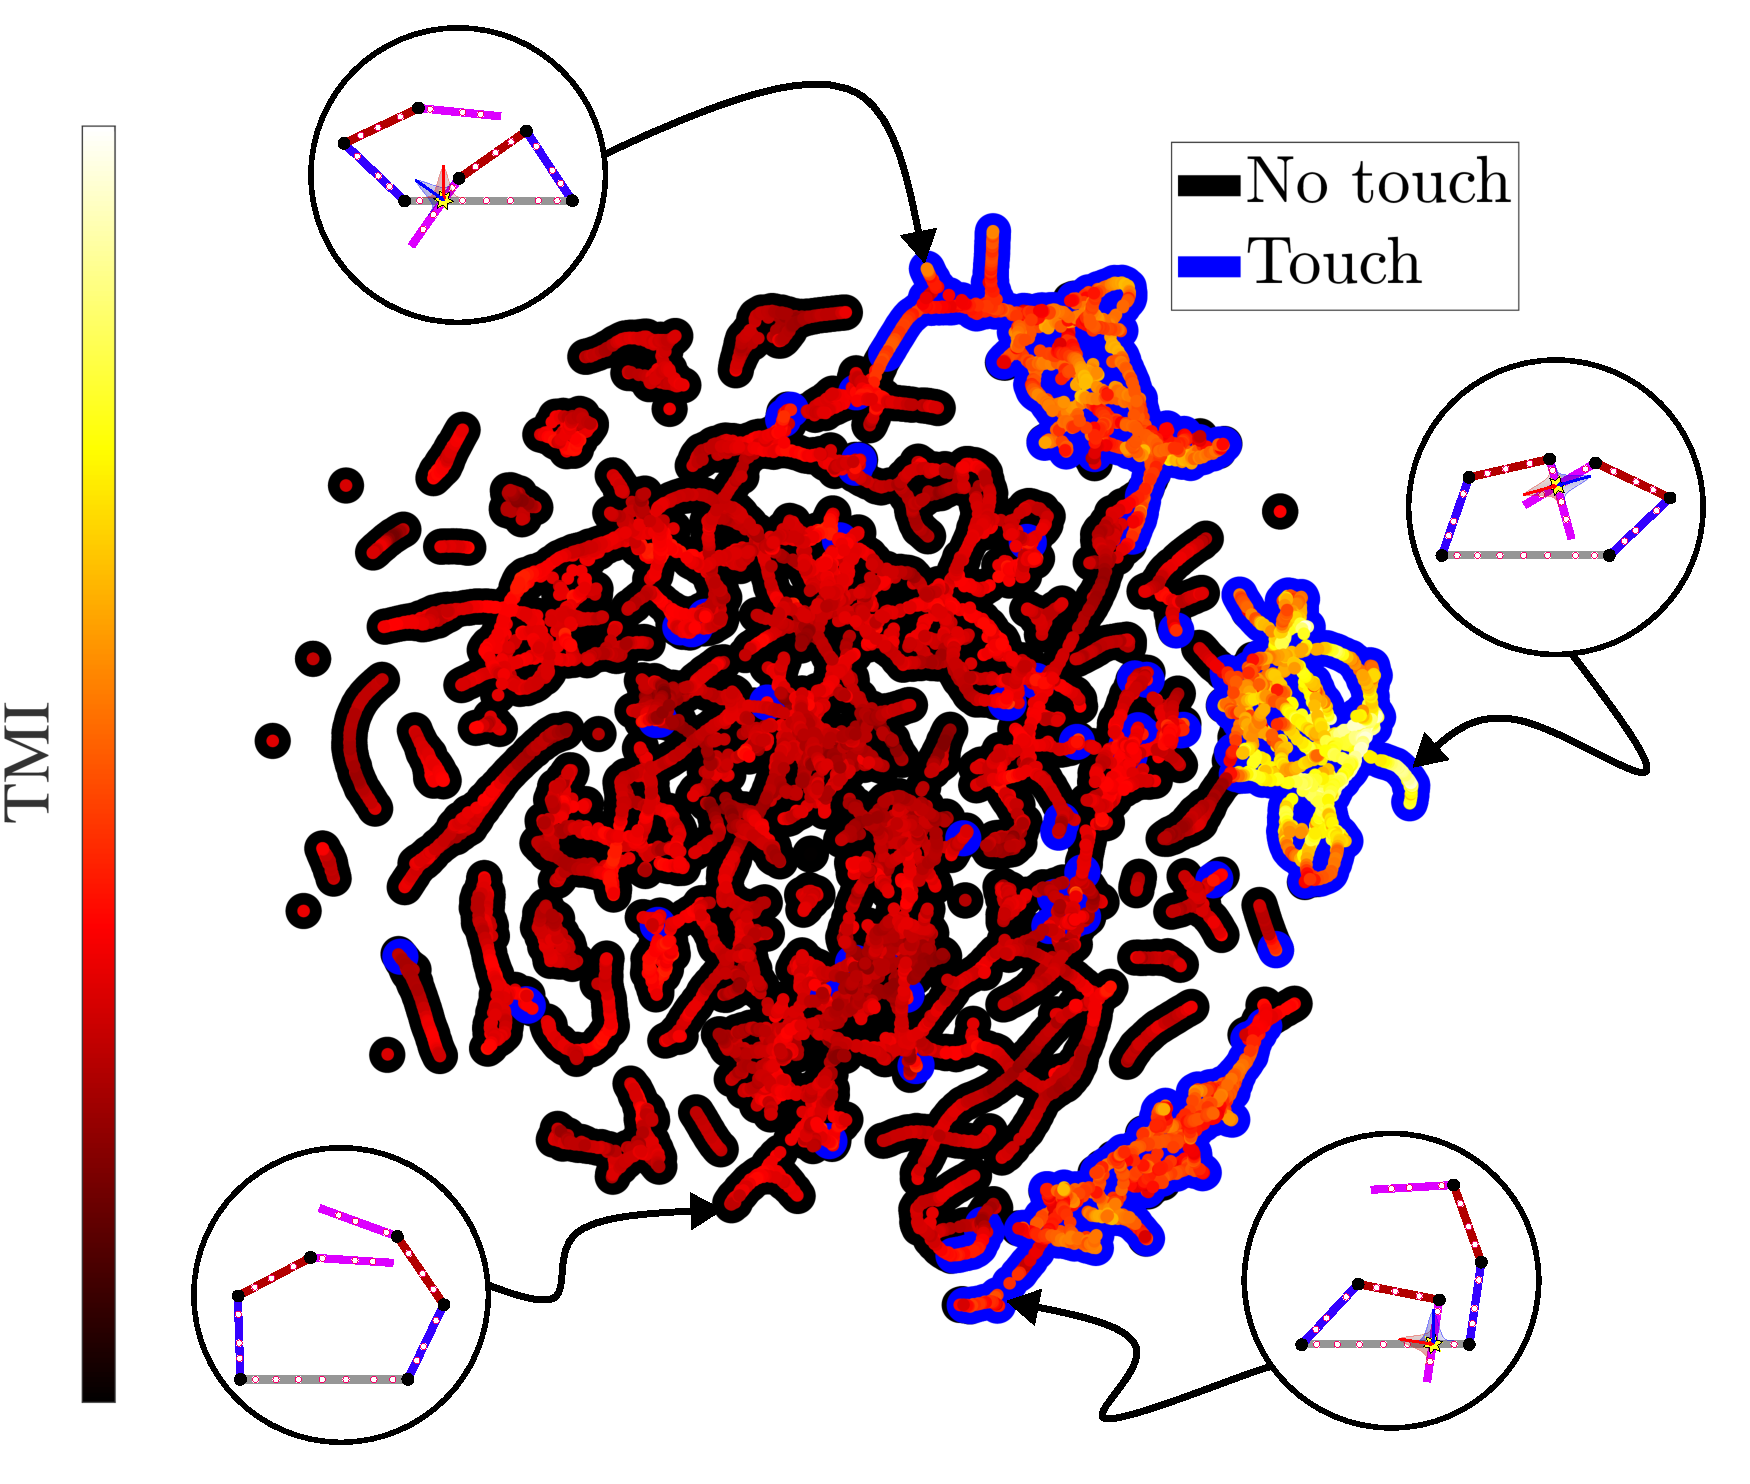
\includegraphics[width=0.99\columnwidth]{fig/pacmac_with_timi_and_modes.pdf}
	\caption{A two dimensional projection using PaCMAP of the coefficients $\bm{H}$. The color of each point is scaled by its total mutual information value.}
	\label{fig:pacmac_with_timi_and_modes}
\end{figure}

% =============================================================================
%                                                                             |
%                                                                             |
% ------------------------------- SECTION ------------------------------------|
%                                                                             |
%                                                                             |
% =============================================================================
\section{Case study: robot excitation trajectories}
\TODO
In this section, we use the instantaneous mutual information to generate trajectories for the left and right arms avoiding potential collisions. This is done agnostic to the actual morphology of the robot. In contrast, we use a standard method for the design of excitation trajectories and compare the results.

% =============================================================================
%                                                                             |
%                                                                             |
% ------------------------------- SECTION ------------------------------------|
%                                                                             |
%                                                                             |
% =============================================================================
\section{Beyond robotics}
\TODO
\myhl{Valentin + Matej}

% =============================================================================
%                                                                             |
%                                                                             |
% ------------------------------- SECTION ------------------------------------|
%                                                                             |
%                                                                             |
% =============================================================================
\section{Conclusions}\label{sec:conclusion}


\section{Discussion and Future Work}


\printbibliography 
\end{document}